\documentclass[10pt, a4paper]{article}\usepackage[]{graphicx}\usepackage[]{xcolor}
% maxwidth is the original width if it is less than linewidth
% otherwise use linewidth (to make sure the graphics do not exceed the margin)
\makeatletter
\def\maxwidth{ %
  \ifdim\Gin@nat@width>\linewidth
    \linewidth
  \else
    \Gin@nat@width
  \fi
}
\makeatother

\definecolor{fgcolor}{rgb}{0.345, 0.345, 0.345}
\newcommand{\hlnum}[1]{\textcolor[rgb]{0.686,0.059,0.569}{#1}}%
\newcommand{\hlstr}[1]{\textcolor[rgb]{0.192,0.494,0.8}{#1}}%
\newcommand{\hlcom}[1]{\textcolor[rgb]{0.678,0.584,0.686}{\textit{#1}}}%
\newcommand{\hlopt}[1]{\textcolor[rgb]{0,0,0}{#1}}%
\newcommand{\hlstd}[1]{\textcolor[rgb]{0.345,0.345,0.345}{#1}}%
\newcommand{\hlkwa}[1]{\textcolor[rgb]{0.161,0.373,0.58}{\textbf{#1}}}%
\newcommand{\hlkwb}[1]{\textcolor[rgb]{0.69,0.353,0.396}{#1}}%
\newcommand{\hlkwc}[1]{\textcolor[rgb]{0.333,0.667,0.333}{#1}}%
\newcommand{\hlkwd}[1]{\textcolor[rgb]{0.737,0.353,0.396}{\textbf{#1}}}%
\let\hlipl\hlkwb

\usepackage{framed}
\makeatletter
\newenvironment{kframe}{%
 \def\at@end@of@kframe{}%
 \ifinner\ifhmode%
  \def\at@end@of@kframe{\end{minipage}}%
  \begin{minipage}{\columnwidth}%
 \fi\fi%
 \def\FrameCommand##1{\hskip\@totalleftmargin \hskip-\fboxsep
 \colorbox{shadecolor}{##1}\hskip-\fboxsep
     % There is no \\@totalrightmargin, so:
     \hskip-\linewidth \hskip-\@totalleftmargin \hskip\columnwidth}%
 \MakeFramed {\advance\hsize-\width
   \@totalleftmargin\z@ \linewidth\hsize
   \@setminipage}}%
 {\par\unskip\endMakeFramed%
 \at@end@of@kframe}
\makeatother

\definecolor{shadecolor}{rgb}{.97, .97, .97}
\definecolor{messagecolor}{rgb}{0, 0, 0}
\definecolor{warningcolor}{rgb}{1, 0, 1}
\definecolor{errorcolor}{rgb}{1, 0, 0}
\newenvironment{knitrout}{}{} % an empty environment to be redefined in TeX

\usepackage{alltt}

\usepackage[top=1 in, bottom = 1 in, left = 1 in, right = 1 in ]{geometry}

\usepackage{amsmath, amssymb, amsfonts}
\usepackage{enumerate}
\usepackage{multirow}
\usepackage{hhline}
\usepackage{array}
\usepackage{longtable}
\usepackage{graphicx}

\title{CC12 Practical Q14}
\author{Ananda Biswas}
\date{}
\IfFileExists{upquote.sty}{\usepackage{upquote}}{}
\begin{document}

\maketitle



$\bullet$ The cost of maintenance of shipping tractors seems to increase with the age of the tractor.
	\begin{enumerate}[(a)]
	\item Fit the model $Y = \beta_0 + \beta_1 X + \epsilon$.
	\item Is the model suitable ?
	
	\end{enumerate}
	
	\vspace{20pt}
	
	\begin{table}[!htbp]
	\def\arraystretch{1.5}
	
	\begin{center}
	\begin{tabular}{|>{\centering}m{2cm}|>{\centering\arraybackslash}m{3cm}|}
	
	
	\hline
	
	Age (Years) & 6 month's cost \\
	
	$x$ & $y$ \\\hline\hline
	
	4.5 & 619 \\
	
	\hline
	
	4.5 & 1049 \\
	
	\hline
	
	4.5 & 1033 \\
	
	\hline
	
	4.0 & 495 \\
	
	\hline
	
	4.0 & 729 \\
	
	\hline
	
	4.0 & 681 \\
	
	\hline
	
	5.0 & 890 \\
	
	\hline
	
	5.0 & 1522 \\
	
	\hline
	
	5.5 & 987 \\
	
	\hline
	
	5.0 & 1194 \\
	
	\hline
	
	0.5 & 163 \\
	
	\hline
	
	0.5 & 182 \\
	
	\hline
	
	6.0 & 764 \\
	
	\hline
	
	6.0 & 1373 \\
	
	\hline
	
	1.0 & 978 \\
	
	\hline
	
	1.0 & 466 \\
	
	\hline 
	
	1.0 & 549 \\
	
	\hline
	
	\end{tabular}
	\end{center}
	
	\end{table}




\newpage


$\bullet$ \textbf{Loading the data-set and other initials}

\begin{knitrout}
\definecolor{shadecolor}{rgb}{0.969, 0.969, 0.969}\color{fgcolor}\begin{kframe}
\begin{alltt}
\hlstd{tractor_maintainance_cost_data} \hlkwb{<-} \hlkwd{read.csv}\hlstd{(}\hlstr{"D:\textbackslash{}\textbackslash{}data_sets\textbackslash{}\textbackslash{}cc12_prac_q14_data.csv"}\hlstd{)}

\hlkwd{dim}\hlstd{(tractor_maintainance_cost_data)}
\end{alltt}
\begin{verbatim}
## [1] 17  2
\end{verbatim}
\begin{alltt}
\hlkwd{names}\hlstd{(tractor_maintainance_cost_data)}
\end{alltt}
\begin{verbatim}
## [1] "years" "cost"
\end{verbatim}
\end{kframe}
\end{knitrout}

\begin{knitrout}
\definecolor{shadecolor}{rgb}{0.969, 0.969, 0.969}\color{fgcolor}\begin{kframe}
\begin{alltt}
\hlstd{tractor_maintainance_cost_data}
\end{alltt}
\begin{verbatim}
##    years cost
## 1    4.5  619
## 2    4.5 1049
## 3    4.5 1033
## 4    4.0  495
## 5    4.0  729
## 6    4.0  681
## 7    5.0  890
## 8    5.0 1522
## 9    5.5  987
## 10   5.0 1194
## 11   0.5  163
## 12   0.5  182
## 13   6.0  764
## 14   6.0 1373
## 15   1.0  978
## 16   1.0  466
## 17   1.0  549
\end{verbatim}
\end{kframe}
\end{knitrout}

\newpage

\begin{knitrout}
\definecolor{shadecolor}{rgb}{0.969, 0.969, 0.969}\color{fgcolor}\begin{kframe}
\begin{alltt}
\hlkwd{library}\hlstd{(tidyverse)}
\end{alltt}


{\ttfamily\noindent\color{warningcolor}{\#\# Warning: package 'tidyverse' was built under R version 4.2.3}}

{\ttfamily\noindent\color{warningcolor}{\#\# Warning: package 'ggplot2' was built under R version 4.2.2}}

{\ttfamily\noindent\color{warningcolor}{\#\# Warning: package 'tibble' was built under R version 4.2.3}}

{\ttfamily\noindent\color{warningcolor}{\#\# Warning: package 'tidyr' was built under R version 4.2.3}}

{\ttfamily\noindent\color{warningcolor}{\#\# Warning: package 'readr' was built under R version 4.2.2}}

{\ttfamily\noindent\color{warningcolor}{\#\# Warning: package 'purrr' was built under R version 4.2.3}}

{\ttfamily\noindent\color{warningcolor}{\#\# Warning: package 'dplyr' was built under R version 4.2.3}}

{\ttfamily\noindent\color{warningcolor}{\#\# Warning: package 'stringr' was built under R version 4.2.3}}

{\ttfamily\noindent\color{warningcolor}{\#\# Warning: package 'forcats' was built under R version 4.2.2}}

{\ttfamily\noindent\color{warningcolor}{\#\# Warning: package 'lubridate' was built under R version 4.2.2}}

{\ttfamily\noindent\itshape\color{messagecolor}{\#\# -- Attaching core tidyverse packages ------------------------ tidyverse 2.0.0 --\\\#\# v dplyr \ \ \ \ 1.1.3 \ \ \ \ v readr \ \ \ \ 2.1.4\\\#\# v forcats \ \ 1.0.0 \ \ \ \ v stringr \ \ 1.5.0\\\#\# v ggplot2 \ \ 3.4.1 \ \ \ \ v tibble \ \ \ 3.2.1\\\#\# v lubridate 1.9.2 \ \ \ \ v tidyr \ \ \ \ 1.3.0\\\#\# v purrr \ \ \ \ 1.0.2 \ \ \ \ \\\#\# -- Conflicts ------------------------------------------ tidyverse\_conflicts() --\\\#\# x dplyr::filter() masks stats::filter()\\\#\# x dplyr::lag() \ \ \ masks stats::lag()\\\#\# i Use the conflicted package (<http://conflicted.r-lib.org/>) to force all conflicts to become errors}}\end{kframe}
\end{knitrout}

\newpage

$\bullet$ \textbf{Scatterplot of Age of Tractor vs 6 month's Maintenance Cost}

\begin{knitrout}
\definecolor{shadecolor}{rgb}{0.969, 0.969, 0.969}\color{fgcolor}\begin{kframe}
\begin{alltt}
\hlstd{tractor_maintainance_cost_data} \hlopt
    \hlkwd{ggplot}\hlstd{(}\hlkwd{aes}\hlstd{(}\hlkwc{x} \hlstd{= years,} \hlkwc{y} \hlstd{= cost))} \hlopt{+} \hlkwd{geom_point}\hlstd{(}\hlkwc{size} \hlstd{=} \hlnum{1.5}\hlstd{,} \hlkwc{col} \hlstd{=} \hlstr{"blue"}\hlstd{)} \hlopt{+}
    \hlkwd{scale_x_discrete}\hlstd{(}\hlkwc{limits} \hlstd{= tractor_maintainance_cost_data}\hlopt{$}\hlstd{years)} \hlopt{+} \hlkwd{labs}\hlstd{(}\hlkwc{x} \hlstd{=} \hlstr{"Age (Years)"}\hlstd{,}
    \hlkwc{y} \hlstd{=} \hlstr{"Cost"}\hlstd{,} \hlkwc{title} \hlstd{=} \hlstr{"Scatterplot of Age vs Cost"}\hlstd{)}
\end{alltt}


{\ttfamily\noindent\color{warningcolor}{\#\# Warning: Continuous limits supplied to discrete scale.\\\#\# i Did you mean `limits = factor(...)` or `scale\_*\_continuous()`?}}\end{kframe}
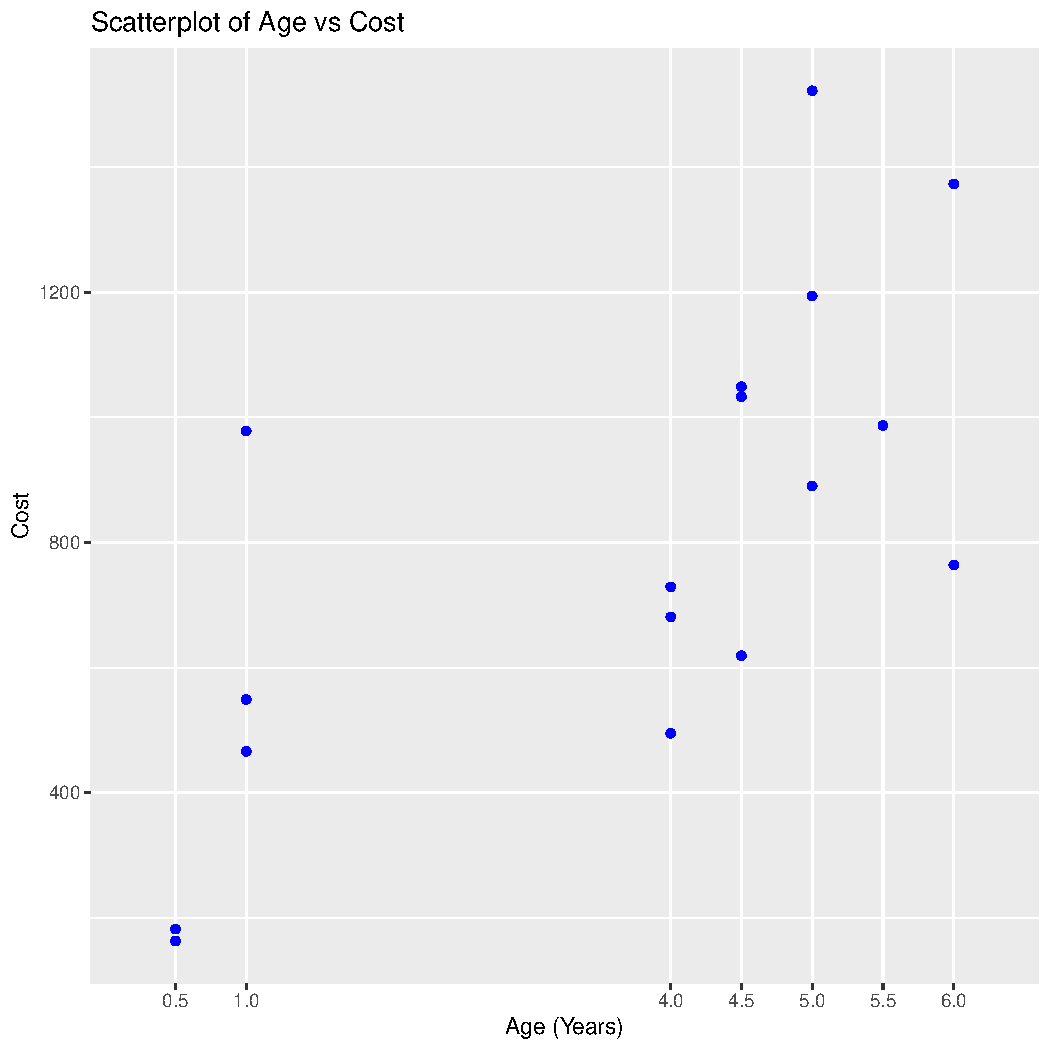
\includegraphics[width=\maxwidth]{figure/unnamed-chunk-4-1} 
\end{knitrout}


\newpage

$\bullet$ \textbf{Test for Normality :: Q-Q Plot}

\begin{knitrout}
\definecolor{shadecolor}{rgb}{0.969, 0.969, 0.969}\color{fgcolor}\begin{kframe}
\begin{alltt}
\hlstd{tractor_maintainance_cost_data} \hlopt
    \hlkwd{ggplot}\hlstd{(}\hlkwd{aes}\hlstd{(}\hlkwc{sample} \hlstd{= cost))} \hlopt{+} \hlkwd{geom_qq}\hlstd{(}\hlkwc{size} \hlstd{=} \hlnum{2}\hlstd{,} \hlkwc{col} \hlstd{=} \hlstr{"blue"}\hlstd{)} \hlopt{+} \hlkwd{geom_qq_line}\hlstd{(}\hlkwc{linewidth} \hlstd{=} \hlnum{1}\hlstd{,}
    \hlkwc{col} \hlstd{=} \hlstr{"red"}\hlstd{)} \hlopt{+} \hlkwd{labs}\hlstd{(}\hlkwc{x} \hlstd{=} \hlstr{"Theoretical Quantiles"}\hlstd{,} \hlkwc{y} \hlstd{=} \hlstr{"Sample Quantiles"}\hlstd{,}
    \hlkwc{title} \hlstd{=} \hlstr{"Q-Q Plot"}\hlstd{)}
\end{alltt}
\end{kframe}
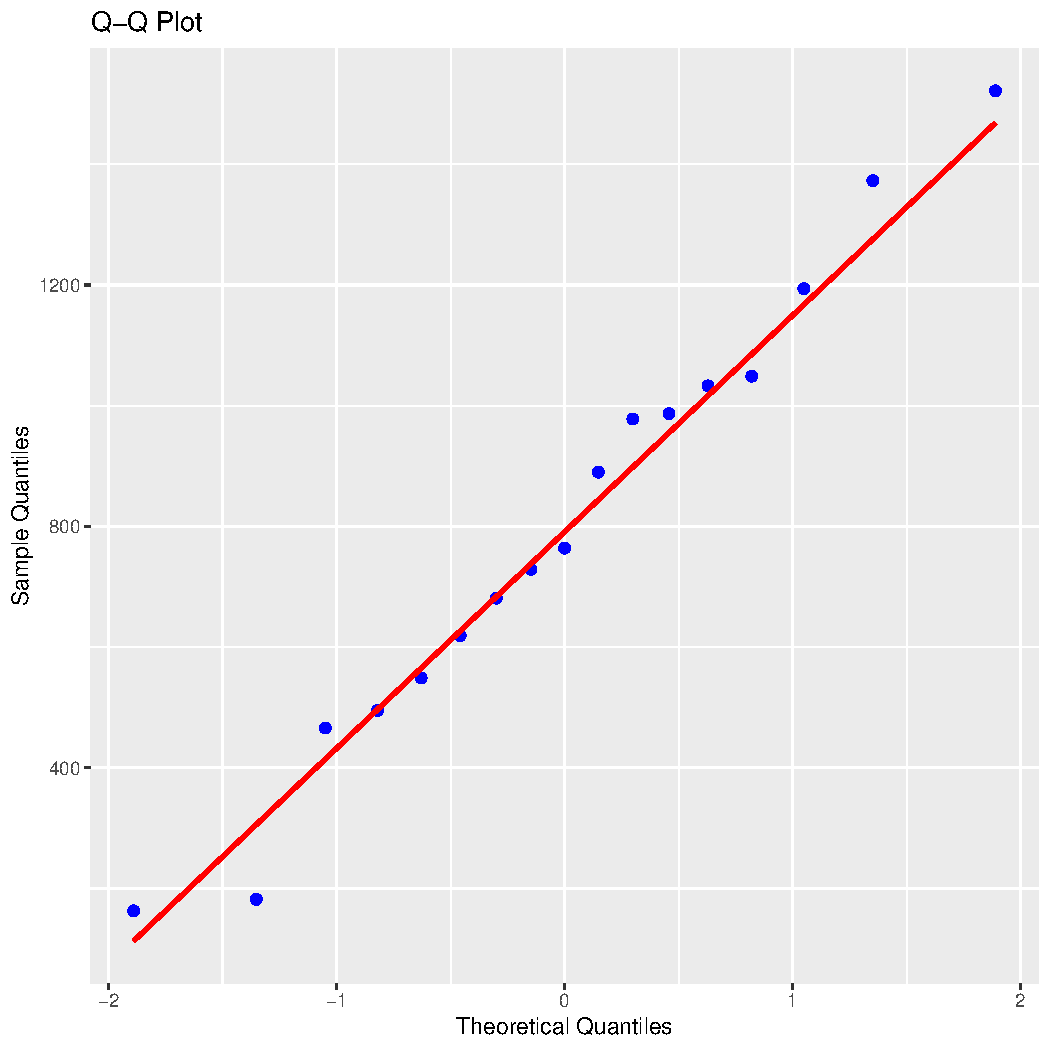
\includegraphics[width=\maxwidth]{figure/unnamed-chunk-5-1} 
\end{knitrout}

We see that it is a good fit. So normality assumption holds.

\newpage

$\bullet$ \textbf{Test for Normality :: Shapiro-Wilk Test}

\begin{knitrout}
\definecolor{shadecolor}{rgb}{0.969, 0.969, 0.969}\color{fgcolor}\begin{kframe}
\begin{alltt}
\hlkwd{shapiro.test}\hlstd{(tractor_maintainance_cost_data}\hlopt{$}\hlstd{cost)}
\end{alltt}
\begin{verbatim}
## 
## 	Shapiro-Wilk normality test
## 
## data:  tractor_maintainance_cost_data$cost
## W = 0.97911, p-value = 0.9485
\end{verbatim}
\end{kframe}
\end{knitrout}

The p-value is much higher than 0.05. So we fail to reject the null hypothesis that the data is sampled from a normal population.



\newpage

\begin{knitrout}
\definecolor{shadecolor}{rgb}{0.969, 0.969, 0.969}\color{fgcolor}\begin{kframe}
\begin{alltt}
\hlstd{fit1} \hlkwb{<-} \hlkwd{lm}\hlstd{(cost} \hlopt{~} \hlstd{years,} \hlkwc{data} \hlstd{= tractor_maintainance_cost_data)}
\end{alltt}
\end{kframe}
\end{knitrout}

Let us have the diagonal elements of the hat matrix.

\begin{knitrout}
\definecolor{shadecolor}{rgb}{0.969, 0.969, 0.969}\color{fgcolor}\begin{kframe}
\begin{alltt}
\hlstd{h} \hlkwb{<-} \hlkwd{hatvalues}\hlstd{(fit1)}
\hlcom{# lm.influence(fit1)$hat}
\hlstd{h}
\end{alltt}
\begin{verbatim}
##          1          2          3          4          5          6          7 
## 0.07030162 0.07030162 0.07030162 0.06078886 0.06078886 0.06078886 0.08770302 
##          8          9         10         11         12         13         14 
## 0.08770302 0.11299304 0.08770302 0.21508121 0.21508121 0.14617169 0.14617169 
##         15         16         17 
## 0.16937355 0.16937355 0.16937355
\end{verbatim}
\end{kframe}
\end{knitrout}

\newpage

$\bullet$ \textbf{Detection of Outliers}

\begin{knitrout}
\definecolor{shadecolor}{rgb}{0.969, 0.969, 0.969}\color{fgcolor}\begin{kframe}
\begin{alltt}
\hlstd{standardised_residuals} \hlkwb{<-} \hlstd{fit1}\hlopt{$}\hlstd{residuals}\hlopt{/}\hlkwd{sqrt}\hlstd{(}\hlkwd{mean}\hlstd{(fit1}\hlopt{$}\hlstd{residuals}\hlopt{^}\hlnum{2}\hlstd{)} \hlopt{*}
    \hlstd{(}\hlnum{1} \hlopt{-} \hlstd{h))}

\hlstd{standardised_residuals}
\end{alltt}
\begin{verbatim}
##          1          2          3          4          5          6          7 
## -1.1603144  0.5154953  0.4531396 -1.3798001 -0.4724779 -0.6585953 -0.3643202 
##          8          9         10         11         12         13         14 
##  2.1221098 -0.2452910  0.8316841 -0.9616580 -0.8810704 -1.4247787  1.0518408 
##         15         16         17 
##  2.1538967  0.0428669  0.3850846
\end{verbatim}
\end{kframe}
\end{knitrout}

\begin{knitrout}
\definecolor{shadecolor}{rgb}{0.969, 0.969, 0.969}\color{fgcolor}\begin{kframe}
\begin{alltt}
\hlkwd{which}\hlstd{(}\hlkwd{abs}\hlstd{(standardised_residuals)} \hlopt{>} \hlnum{3}\hlstd{)}
\end{alltt}
\begin{verbatim}
## named integer(0)
\end{verbatim}
\end{kframe}
\end{knitrout}

None of the absolute values of the standardized residuals is more than 3. So we drop of the suspicion of presence of any outlier.

\newpage

$\bullet$ \textbf{Detection of High Leverage Observations}

\begin{knitrout}
\definecolor{shadecolor}{rgb}{0.969, 0.969, 0.969}\color{fgcolor}\begin{kframe}
\begin{alltt}
\hlkwd{which}\hlstd{(h} \hlopt{>} \hlstd{(}\hlnum{3} \hlopt{*} \hlnum{1}\hlstd{)}\hlopt{/}\hlnum{17}\hlstd{)}
\end{alltt}
\begin{verbatim}
## 11 12 
## 11 12
\end{verbatim}
\end{kframe}
\end{knitrout}

So 11th and 12th value of the covariate(here years) are high leverage observations.

\begin{knitrout}
\definecolor{shadecolor}{rgb}{0.969, 0.969, 0.969}\color{fgcolor}\begin{kframe}
\begin{alltt}
\hlstd{tractor_maintainance_cost_data[}\hlkwd{which}\hlstd{(h} \hlopt{>} \hlstd{(}\hlnum{3} \hlopt{*} \hlnum{1}\hlstd{)}\hlopt{/}\hlnum{17}\hlstd{),} \hlnum{1}\hlstd{]}
\end{alltt}
\begin{verbatim}
## [1] 0.5 0.5
\end{verbatim}
\end{kframe}
\end{knitrout}

\newpage

$\bullet$ \textbf{Detection of Influential Observations}

\begin{knitrout}
\definecolor{shadecolor}{rgb}{0.969, 0.969, 0.969}\color{fgcolor}\begin{kframe}
\begin{alltt}
\hlstd{cooks_distance} \hlkwb{<-} \hlkwd{cooks.distance}\hlstd{(fit1)}

\hlstd{cooks_distance}
\end{alltt}
\begin{verbatim}
##            1            2            3            4            5            6 
## 0.0449145449 0.0088651274 0.0068501419 0.0543632563 0.0063743541 0.0123854097 
##            7            8            9           10           11           12 
## 0.0056293342 0.1909969103 0.0033814278 0.0293364438 0.1117973181 0.0938450259 
##           13           14           15           16           17 
## 0.1533203953 0.0835612786 0.4173514264 0.0001653089 0.0133402667
\end{verbatim}
\end{kframe}
\end{knitrout}

\begin{knitrout}
\definecolor{shadecolor}{rgb}{0.969, 0.969, 0.969}\color{fgcolor}\begin{kframe}
\begin{alltt}
\hlkwd{which}\hlstd{(cooks_distance} \hlopt{>} \hlnum{4}\hlopt{/}\hlnum{17}\hlstd{)}
\end{alltt}
\begin{verbatim}
## 15 
## 15
\end{verbatim}
\end{kframe}
\end{knitrout}

So 15th observation is an influential observation.

\begin{knitrout}
\definecolor{shadecolor}{rgb}{0.969, 0.969, 0.969}\color{fgcolor}\begin{kframe}
\begin{alltt}
\hlstd{tractor_maintainance_cost_data[}\hlkwd{which}\hlstd{(cooks_distance} \hlopt{>} \hlnum{4}\hlopt{/}\hlnum{17}\hlstd{), ]}
\end{alltt}
\begin{verbatim}
##    years cost
## 15     1  978
\end{verbatim}
\end{kframe}
\end{knitrout}


\newpage

$\bullet$ \textbf{Test for Homoscedasticity :: Goldfeld-Quandt Test}

\begin{knitrout}
\definecolor{shadecolor}{rgb}{0.969, 0.969, 0.969}\color{fgcolor}\begin{kframe}
\begin{alltt}
\hlkwd{library}\hlstd{(lmtest)}
\end{alltt}


{\ttfamily\noindent\color{warningcolor}{\#\# Warning: package 'lmtest' was built under R version 4.2.3}}

{\ttfamily\noindent\itshape\color{messagecolor}{\#\# Loading required package: zoo}}

{\ttfamily\noindent\itshape\color{messagecolor}{\#\# \\\#\# Attaching package: 'zoo'}}

{\ttfamily\noindent\itshape\color{messagecolor}{\#\# The following objects are masked from 'package:base':\\\#\# \\\#\# \ \ \ \ as.Date, as.Date.numeric}}\end{kframe}
\end{knitrout}

\begin{knitrout}
\definecolor{shadecolor}{rgb}{0.969, 0.969, 0.969}\color{fgcolor}\begin{kframe}
\begin{alltt}
\hlkwd{gqtest}\hlstd{(fit1,} \hlkwc{order.by} \hlstd{=} \hlopt{~}\hlstd{years,} \hlkwc{data} \hlstd{= tractor_maintainance_cost_data)}
\end{alltt}
\begin{verbatim}
## 
## 	Goldfeld-Quandt test
## 
## data:  fit1
## GQ = 1.2262, df1 = 7, df2 = 6, p-value = 0.4098
## alternative hypothesis: variance increases from segment 1 to 2
\end{verbatim}
\end{kframe}
\end{knitrout}

p-value is much higher than 0.05. So we fail to reject the null hypothesis that homoscedasticity is present.


\vspace{50pt}

$\bullet$ \textbf{Test for Homoscedasticity :: Breusch-Pagan Test}

\begin{knitrout}
\definecolor{shadecolor}{rgb}{0.969, 0.969, 0.969}\color{fgcolor}\begin{kframe}
\begin{alltt}
\hlkwd{library}\hlstd{(lmtest)}
\end{alltt}
\end{kframe}
\end{knitrout}

\begin{knitrout}
\definecolor{shadecolor}{rgb}{0.969, 0.969, 0.969}\color{fgcolor}\begin{kframe}
\begin{alltt}
\hlkwd{bptest}\hlstd{(fit1)}
\end{alltt}
\begin{verbatim}
## 
## 	studentized Breusch-Pagan test
## 
## data:  fit1
## BP = 0.0030494, df = 1, p-value = 0.956
\end{verbatim}
\end{kframe}
\end{knitrout}

p-value is much higher than 0.05. So we fail to reject the null hypothesis that homoscedasticity is present.

\newpage

$\bullet$ \textbf{Test for Auto-correlation :: Durbin-Watson Test}

\begin{knitrout}
\definecolor{shadecolor}{rgb}{0.969, 0.969, 0.969}\color{fgcolor}\begin{kframe}
\begin{alltt}
\hlkwd{library}\hlstd{(car)}
\end{alltt}


{\ttfamily\noindent\itshape\color{messagecolor}{\#\# Loading required package: carData}}

{\ttfamily\noindent\itshape\color{messagecolor}{\#\# \\\#\# Attaching package: 'car'}}

{\ttfamily\noindent\itshape\color{messagecolor}{\#\# The following object is masked from 'package:dplyr':\\\#\# \\\#\# \ \ \ \ recode}}

{\ttfamily\noindent\itshape\color{messagecolor}{\#\# The following object is masked from 'package:purrr':\\\#\# \\\#\# \ \ \ \ some}}\end{kframe}
\end{knitrout}

\begin{knitrout}
\definecolor{shadecolor}{rgb}{0.969, 0.969, 0.969}\color{fgcolor}\begin{kframe}
\begin{alltt}
\hlkwd{durbinWatsonTest}\hlstd{(fit1)}
\end{alltt}
\begin{verbatim}
##  lag Autocorrelation D-W Statistic p-value
##    1      0.03418094      1.850764   0.642
##  Alternative hypothesis: rho != 0
\end{verbatim}
\end{kframe}
\end{knitrout}

p-value is much higher than 0.05. So we fail to reject the null hypothesis that the residuals are not auto-correlated.

\newpage

\begin{knitrout}
\definecolor{shadecolor}{rgb}{0.969, 0.969, 0.969}\color{fgcolor}\begin{kframe}
\begin{alltt}
\hlkwd{summary}\hlstd{(fit1)}
\end{alltt}
\begin{verbatim}
## 
## Call:
## lm(formula = cost ~ years, data = tractor_maintainance_cost_data)
## 
## Residuals:
##     Min      1Q  Median      3Q     Max 
## -355.85 -207.73  -61.48  132.27  539.40 
## 
## Coefficients:
##             Estimate Std. Error t value Pr(>|t|)   
## (Intercept)   323.85     146.85   2.205  0.04345 * 
## years         131.75      35.59   3.702  0.00213 **
## ---
## Signif. codes:  0 '***' 0.001 '**' 0.01 '*' 0.05 '.' 0.1 ' ' 1
## 
## Residual standard error: 283.3 on 15 degrees of freedom
## Multiple R-squared:  0.4775,	Adjusted R-squared:  0.4427 
## F-statistic: 13.71 on 1 and 15 DF,  p-value: 0.002129
\end{verbatim}
\end{kframe}
\end{knitrout}

\newpage

$\bullet$ \textbf{Residual Plot}

\begin{knitrout}
\definecolor{shadecolor}{rgb}{0.969, 0.969, 0.969}\color{fgcolor}\begin{kframe}
\begin{alltt}
\hlstd{df1} \hlkwb{<-} \hlkwd{data.frame}\hlstd{(}\hlkwc{sample_no} \hlstd{=} \hlnum{1}\hlopt{:}\hlkwd{length}\hlstd{(fit1}\hlopt{$}\hlstd{residuals),} \hlkwc{residuals} \hlstd{= fit1}\hlopt{$}\hlstd{residuals)}
\end{alltt}
\end{kframe}
\end{knitrout}

\begin{knitrout}
\definecolor{shadecolor}{rgb}{0.969, 0.969, 0.969}\color{fgcolor}\begin{kframe}
\begin{alltt}
\hlstd{df1} \hlopt
    \hlkwd{ggplot}\hlstd{(}\hlkwd{aes}\hlstd{(}\hlkwc{x} \hlstd{= sample_no,} \hlkwc{y} \hlstd{= residuals))} \hlopt{+} \hlkwd{geom_point}\hlstd{(}\hlkwc{size} \hlstd{=} \hlnum{1.5}\hlstd{,}
    \hlkwc{col} \hlstd{=} \hlstr{"red"}\hlstd{)} \hlopt{+} \hlkwd{geom_hline}\hlstd{(}\hlkwc{yintercept} \hlstd{=} \hlnum{0}\hlstd{,} \hlkwc{linewidth} \hlstd{=} \hlnum{1}\hlstd{,} \hlkwc{col} \hlstd{=} \hlstr{"blue"}\hlstd{)} \hlopt{+}
    \hlkwd{scale_x_discrete}\hlstd{(}\hlkwc{limits} \hlstd{=} \hlnum{1}\hlopt{:}\hlkwd{length}\hlstd{(fit1}\hlopt{$}\hlstd{residuals))} \hlopt{+} \hlkwd{labs}\hlstd{(}\hlkwc{x} \hlstd{=} \hlstr{"Observation Number"}\hlstd{,}
    \hlkwc{y} \hlstd{=} \hlstr{"Residual"}\hlstd{,} \hlkwc{title} \hlstd{=} \hlstr{"Residual Plot"}\hlstd{)}
\end{alltt}


{\ttfamily\noindent\color{warningcolor}{\#\# Warning: Continuous limits supplied to discrete scale.\\\#\# i Did you mean `limits = factor(...)` or `scale\_*\_continuous()`?}}\end{kframe}
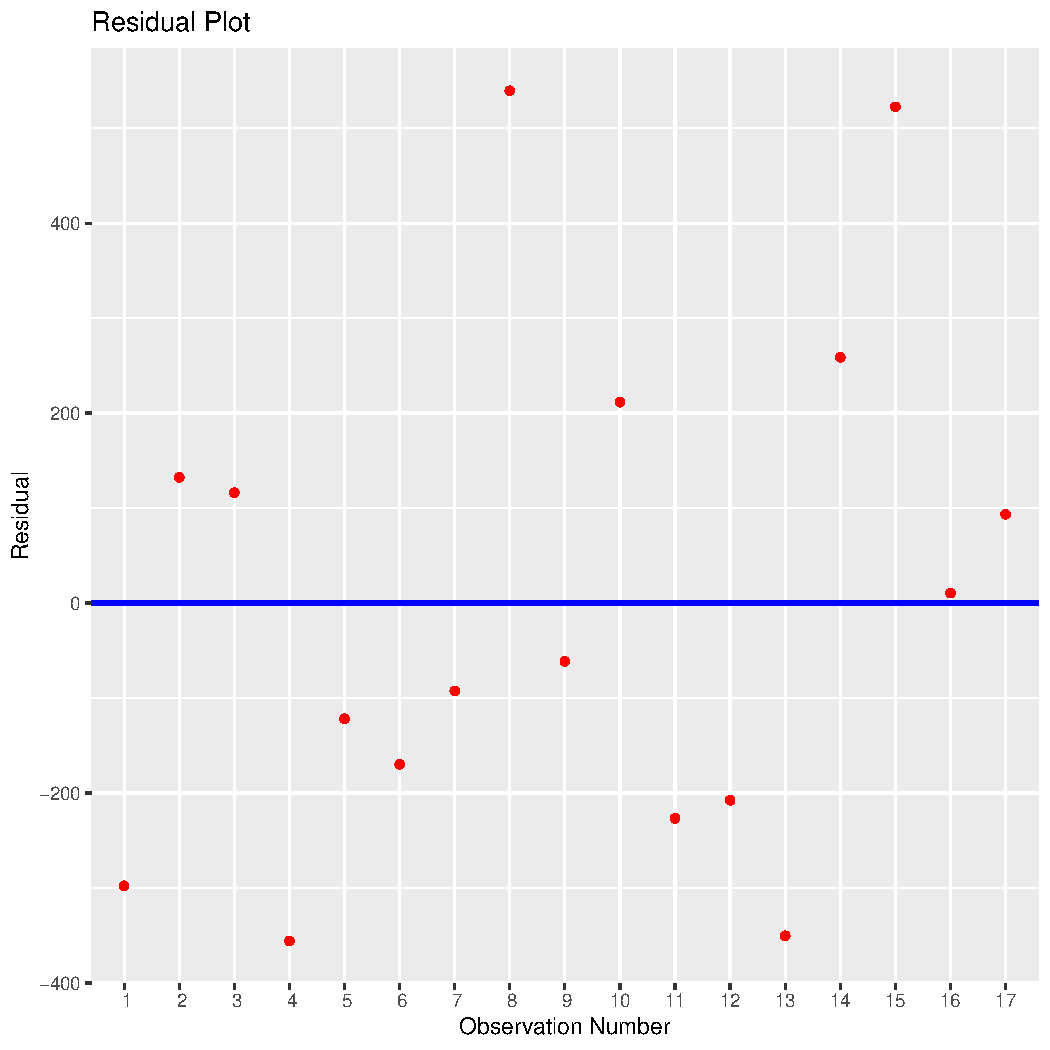
\includegraphics[width=\maxwidth]{figure/unnamed-chunk-24-1} 
\end{knitrout}


\newpage

$\bullet$ \textbf{Model Checking}

Let us have a look at R-squared for the model.
\begin{knitrout}
\definecolor{shadecolor}{rgb}{0.969, 0.969, 0.969}\color{fgcolor}\begin{kframe}
\begin{alltt}
\hlkwd{summary}\hlstd{(fit1)}\hlopt{$}\hlstd{r.squared}
\end{alltt}
\begin{verbatim}
## [1] 0.4774928
\end{verbatim}
\end{kframe}
\end{knitrout}

Let us have a look at Adjusted R-squared for the model.
\begin{knitrout}
\definecolor{shadecolor}{rgb}{0.969, 0.969, 0.969}\color{fgcolor}\begin{kframe}
\begin{alltt}
\hlkwd{summary}\hlstd{(fit1)}\hlopt{$}\hlstd{adj.r.squared}
\end{alltt}
\begin{verbatim}
## [1] 0.4426589
\end{verbatim}
\end{kframe}
\end{knitrout}


\end{document}
